\documentclass[a4paper, oneside, 12pt]{article}

% Layout
%\usepackage[top=2.54cm, bottom=3.04cm, left=2.74cm, right=2.75cm]{geometry}
%\usepackage{parskip}

% Font
\usepackage[T1]{fontenc}
\usepackage{helvet}
\usepackage{upquote}

\renewcommand*\familydefault{\sfdefault}

% Graphics
\usepackage{graphicx}
\usepackage{subcaption}
\usepackage{xcolor}

\usepackage{tikz}
\usepackage[oldvoltagedirection]{circuitikz}

\usepackage{pgfplots}

% Math
\usepackage{amsmath, amsfonts, mathtools, amsthm, amssymb}
\usepackage{unicode-math}
\usepackage{bm} 		% Bold math
\usepackage{nicefrac}

\AtBeginDocument{
	\renewcommand{\vec}[1]{\mathbf{#1}}
}

\newcommand{\vecr}{\ensuremath{\vec{r}}}
\newcommand{\vecrp}{\ensuremath{\vec{r}^\prime}}

\newcommand{\oL}{\mathcal{L}}

% SI units
\usepackage{siunitx}
\sisetup{
	range-units = single,
	range-phrase = {--},
	per-mode = symbol,
	per-symbol = {/},
	bracket-unit-denominator = true,
	list-units = single,
	list-final-separator = { en },
	list-pair-separator = { en }
}

% Packages
\usepackage{textcomp}
\usepackage{url}
\usepackage{hyperref}

\hypersetup{
	colorlinks,
	linkcolor = {black!50!black},
	citecolor = {blue!50!black},
	urlcolor = {blue!80!black}
}

\title{The Method of Moments\\for Antenna Simulation}
\author{Gijs Lagerweij}

\begin{document}
	\maketitle
	
	\tableofcontents
	
	\clearpage
\section{Introduction}
In this document, we present a derivation of the method of moments (MoM) applied to antenna modelling. It is intended for readers with a background in electromagnetics who want to understand the theory behind the MoM and its application in antenna design.

The primary objective is to simulate the impedance and far-field radiation patterns of antennas made from thin wires, particularly those where the wire diameter is much smaller than the wavelength of operation. These types of antennas are commonly found in consumer electronics and amateur radio systems, among other applications. The document not only lays out the theoretical foundations but also demonstrates the application of the MoM through several practical examples, which are available in the GitHub repository:
\begin{itemize}
	\item Center-fed half-wave dipoles,
	\item End-fed half-wave antennas,
	\item Antennas with parasitic elements, such as Yagi-Uda arrays,
	\item Loop antennas.
\end{itemize}

We begin with Maxwell's equations and derive an integral equation for the electric field in free space. We then apply the Method of Moments to discretize this integral equation using triangular basis functions. This process results in a solvable system of linear equations. From the solution, we can calculate our desired quantities, such as impedance and radiated power.
	\section{Electromagnetic Theory}

\subsection{Maxwell's Equations}
In a homogeneous region with permittivity $\varepsilon$ and permeability $\mu$, Maxwell's equations describe the electric fields $\vec{E}, \vec{D}$ and magnetic fields $\vec{H}, \vec{B}$.
\begin{align}
	\nabla \times \vec{E} & = -j\omega\mu\vec{H}, \label{eq:maxwell_E} \\
	\nabla \times \vec{H} & = j\omega\varepsilon\vec{E} + \vec{J}_0, \label{eq:maxwell_H} \\
	\nabla \cdot \vec{D} & = \rho, \label{eq:maxwell_D} \\
	\nabla \cdot \vec{B} & = 0, \label{eq:maxwell_B}
\end{align}
where $\vec{B} = \mu \vec{H}$ and $\vec{D} = \varepsilon \vec{E}$. Throughout the text, we assume a time-harmonic formulation with time dependence $e^{j\omega t}$.

\subsection{Green's Functions}
A Green's function is the impulse response of a linear differential equations on a specified domain. Using the superposition principle, the solution of a differential equation can be expressed as a sum of Green's functions. This property will allow us to write an integral equation for the electric field in Section~\ref{sec:em_efie}.

\subsubsection{Electrostatic Green's Function}
Consider the electrostatic Poisson equation
\begin{equation}
	\nabla^2 \phi = -\frac{\rho}{\varepsilon},
\end{equation}
where $\rho$ is the charge density. We can apply the Green's function method as outlined above to find the electric potential due to an arbitrary charge configuration. First, we find the impulse response $G(r)$ such that
\begin{equation}
	\nabla^2 G(\vecr) = -\frac{\delta(\vecr)}{\varepsilon}.
\end{equation}
Expanding the Laplace operator in spherical coordinates, we find
\begin{equation*}
	\nabla^2 G = \frac{1}{r^2} \frac{\partial}{\partial r} \left[ r^2 \frac
	{\partial G}{\partial r} \right] = \frac{\partial^2 G}{\partial r^2} + \frac{2}{r} \frac{\partial G}{\partial r} = \frac{1}{r} \frac{\partial^2 (r G)}{\partial r^2}
\end{equation*}
Outside of the point $r = 0$, the Dirac delta function is zero, such that
\begin{equation}
	\frac{\partial^2 (r G)}{\partial r^2} = 0 \qquad r > 0
\end{equation}
Integrating this differential equation twice gives us the general solution $G(r) = a + \frac{b}{r}$. We must have $G \to 0$ as $r \to \infty$, so the coefficient $a = 0$. To find coefficient $b$, we integrate the differential equation over a sphere of radius $R$:
\begin{align*}
	b \iiint_{V} \nabla^2 \left( \frac{1}{r} \right) dV & = - \iiint_V \frac{\delta(r)}{\varepsilon} dV = -\frac{1}{\varepsilon} \\
	\oiint_{\partial V} \nabla \left( \frac{1}{r} \right) \cdot \hat{\vecr} ds & = -\frac{1}{\varepsilon b} \\
	\oiint_{\partial V} \frac{1}{r^2} ds & = \frac{1}{\varepsilon b} \\
	4\pi & = \frac{1}{\varepsilon b}
\end{align*}
Therefore, the electrostatic Green's function becomes
\begin{equation}
	G(\vecr, \vecrp) = \frac{1}{4\pi \varepsilon r}, \qquad r = |\vecr - \vecrp|.
\end{equation}
Then, the electric potential due to an arbitrary charge distribution $\rho(\vecr)$ is 
\begin{equation}
	\phi(\vecr) = \iiint G(\vecr, \vecrp) \rho(\vecrp) d\vecrp = \frac{1}{4\pi\varepsilon} \iiint \frac{\rho(\vecrp)}{|\vecr - \vecrp|} d\vecrp
\end{equation}

\subsubsection{Electrodynamic Green's Function}
Similarly, we can derive a Green's function which satisfies the scalar Helmholtz equation. It will be shown later that the electrodynamic equations resemble the (vector) Helmholtz equation. Consider
\begin{equation}
	\nabla^2 G(\vecr, \vecrp) + k^2 G(\vecr, \vecrp) = -\delta(\vecr, \vecrp)
\end{equation}
Using the same derivation as before, we can equate the left-hand side to zero for $r > 0$.
\begin{equation}
	\frac{\partial^2 (r G)}{\partial r^2} + k^2 (r G) = 0 \qquad r > 0
\end{equation}
The solution to this differential equation is
\begin{equation*}
	G(r) = \frac{a e^{-j k r}}{r} + \frac{b e^{+j k r}}{r}.
\end{equation*}
By requiring that $G \to 0$ as $r \to \infty$, we find that $b = 0$. To find coefficient $a$, we again integrate over a sphere of radius $R$.
\begin{equation*}
	a \iiint_V \nabla^2 \left( \frac{e^{-jkr}}{r} \right) + k^2 \left( \frac{e^{-jkr}}{r} \right) dV = -1
\end{equation*}
The first part of the integral can be tackled by applying the divergence theorem:
\begin{align*}
	\iiint_V \nabla^2 \left( \frac{e^{-jkr}}{r} \right) dV & = \oiint_{\partial V} \nabla \left( \frac{e^{-jkr}}{r} \right) \cdot \hat{\vecr} ds = 4\pi a^2 \left[ \frac{\partial}{\partial r} \left( \frac{e^{-jkr}}{r} \right) \right]_{r = R} \\
	\lim_{R \to 0} 4\pi a^2 \left[ \frac{\partial}{\partial r} \left( \frac{e^{-jkr}}{r} \right) \right]_{r = R} & = -4\pi
\end{align*}
The second part of the integral is calculated by inspection:
\begin{align*}
	\iiint_V k^2 \left( \frac{e^{-jkr}}{r} \right) dV & = 4\pi k^2 R^2 \int_0^R \frac{e^{-jkr}}{r} dr \\
	\lim_{R \to 0} 4\pi k^2 R^2 \int_0^R \frac{e^{-jkr}}{r} dr & = 0
\end{align*}
Therefore, we find that the coefficient $a = \frac{1}{4\pi}$ and the electrodynamic Green's function is
\begin{equation}
	G(\vecr, \vecrp) = \frac{e^{-jkr}}{4\pi r}, \qquad r = |\vecr - \vecrp|.
\end{equation}

\subsection{Electric Field Integral Equation (EFIE)}
\label{sec:em_efie}
Taking the curl of (\ref{eq:maxwell_E}) we obtain
\begin{equation*}
	\nabla \times \nabla \times \vec{E}  = -j\omega\mu (j\omega\varepsilon \vec{E} + \vec{J}) = \nabla (\nabla \cdot \vec{E}) - \nabla^2 \vec{E}
\end{equation*}
Gathering the unknown $\vec{E}$ on the left-hand side, and the source terms involving $\vec{J}$ on the right:
\begin{equation}
	\nabla^2 \vec{E} + k^2 \vec{E} = j\omega\mu\vec{J} - \frac{\nabla (\nabla \cdot \vec{J})}{j\omega\varepsilon}
\end{equation}
This equation has the vector Helmholtz form with wavenumber $k = \nicefrac{\omega}{c} = \omega \sqrt{\mu \varepsilon}$. Using the electrodynamic Green's function derived above, we get an integral equation for the electric field.
\begin{equation}
	\vec{E}(\vecr) = -j\omega\mu \iiint G(\vecr, \vecrp) \left[ 1 + \frac
	{\nabla^\prime \nabla^\prime}{k^2} \right] \vec{J}(\vecrp) d\vecrp
	\label{eq:efie}
\end{equation}
Equation (\ref{eq:efie}) is called the \emph{electric field integral equation} (EFIE) and can also be written more compactly in terms of the operator $\oL$.
\begin{equation}
	\vec{E}(\vecr) = -j\omega\mu (\oL \vec{J})(\vecr),
\end{equation}
where
\begin{equation}
	(\oL\vec{X})(\vecr) = \iiint G(\vecr, \vecrp) \left[ 1 + \frac{\nabla^\prime \nabla^\prime}{k^2} \right] \vec{X}(\vecrp) d\vecrp
\end{equation}
Let the total electric field be written as a combination of the scattered field (due to an induced current density $\vec{J}$) and the incident field: $\vec{E} = \vec{E}^{s} + \vec{E}^{i}$. At the boundary of a conducting surface $S$, the following holds:
\begin{equation}
	\hat{\vec{n}}(\vecr) \times \left[ \vec{E}^i(\vecr) + \vec{E}^s(\vecr) \right] = 0,
\end{equation}
where $\hat{\vec{n}}(\vecr)$ is the surface normal at $\vecr \in S$. Thus, we can rewrite the ``surface'' integral equation as
\begin{equation}
	-\hat{\vec{n}}(\vecr) \times \vec{E}^i(\vecr) = \hat{\vec{n}}(\vecr) \times -j\omega\mu(\oL \vec{J})(\vecr)
\end{equation}
Finally, we can drop the $\hat{\vec{n}} \times$ and implicitly assume that the vectorial quantities are tangential to the conducting surface.
\begin{equation}
	\vec{E}^i(\vecr) = j\omega\mu(\oL \vec{J})(\vecr)
	\label{eq:surf_efie}
\end{equation}
Observe that this equation is very similar to the original EFIE in (\ref{eq:efie}), but with a reversed sign. The domain of integration is now restricted to the conducting surfaces.
	\section{Method of Moments}

\subsection{Discretization}
Starting from the EFIE, we expand the unknown current distribution $\vec{J}(\vecr)$ into a series of basis functions:
\begin{equation}
	\vec{J}(\vecr) = \sum_{n = 1}^{N} I_n \vec{f}_n(\vecr),
	\label{eq:j_exp}
\end{equation}
where $I_n$ are the unknown coefficients representing the current, and $\vec{f}_n(\vecr)$ are the vector basis functions. Many choices of basis  are possible, but we will use the triangular basis functions shown in Figure~\ref{fig:mom_basis}. The orientation of the basis vectors is further discussed in Section~\ref{sec:mom_bc}.
\begin{figure}[!ht]
	\centering
	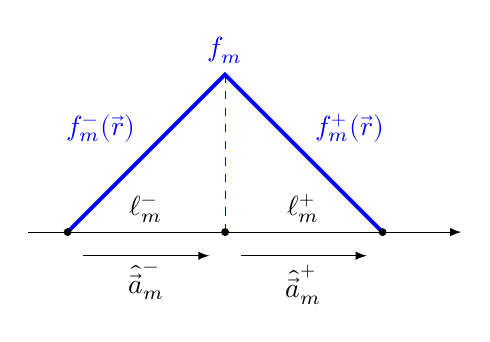
\begin{tikzpicture}[> = latex]
	\draw[->] (-0.5, 0) -- (5, 0);	
	
	\draw[blue, line width=0.5mm] (0, 0) -- node[above left] {$f_m^{-}(\vecr)$} (2, 2) node[above] {$f_m$} -- node[above right] {$f_m^{+}(\vecr)$} (4, 0);
	\draw[blue, dashed] (2, 0) -- (2, 2);
	\node[fill = black, circle, inner sep=0pt, minimum size = 1mm] at (0, 0) {};
	\node[fill = black, circle, inner sep=0pt, minimum size = 1mm] at (2, 0) {};
	\node[fill = black, circle, inner sep=0pt, minimum size = 1mm] at (4, 0) {};
	
	\draw (1, 0) node[above] {$\ell_m^{-}$};
	\draw (3, 0) node[above] {$\ell_m^{+}$};
	
	\draw[->] (0.2, -0.3) -- node[below] {$\hat{\vec{a}}_m^{-}$} (1.8, -0.3);
	\draw[->] (2.2, -0.3) -- node[below] {$\hat{\vec{a}}_m^{+}$} (3.8, -0.3);
\end{tikzpicture}
	\caption{Triangular basis function}
	\label{fig:mom_basis}
\end{figure}

Substituting (\ref{eq:j_exp}) into the EFIE, the $\oL$ operator now operates on the (known) basis functions.
\begin{equation}
	\vec{E}(\vecr) = j\omega\mu \sum_{n = 1}^{N} I_n (\oL \vec{f}_n)(\vecr)
	\label{eq:efie_exp}
\end{equation}
Next, we can test (\ref{eq:efie_exp}) with the same basis functions $\vec{f}_m(\vecr)$ with $m = 1, \dots, N$.
\begin{equation}
	\langle \vec{f}_m, \vec{E} \rangle = j\omega\mu \sum_{n = 1}^{N} I_n \langle \vec{f}_m, \oL \vec{f}_n \rangle \qquad m = 1, \dots, N
\end{equation}
This results in a square $N \times N$ system of equations.
\begin{equation}
	\begin{Bmatrix}
		V
	\end{Bmatrix} = \begin{bmatrix}
		Z
	\end{bmatrix} \begin{Bmatrix}
		I
	\end{Bmatrix},
\end{equation}
with
\begin{align*}
	V_m & = \int_{f_m} \vec{f}_m(\vecr) \cdot \vec{E}(\vecr) d\vecr \\
	Z_{mn} & = j\omega\mu \int_{f_m} \int_{f_n} \vec{f}_m(\vecr) \cdot \vec{f}_n(\vecrp) G_k(\vecr, \vecrp) d\vecrp d\vecr \\
	 & - \frac{1}{j\omega} \int_{f_m} \int_{f_n} \nabla \cdot \vec{f}_m(\vecr) \nabla^\prime \cdot \vec{f}_n(\vecrp) G_k(\vecr, \vecrp) d\vecrp d\vecr
\end{align*}
For ease of notation and to clarify the physical role each integral term plays, we redefine the impedance contribution in terms of the vector potential $\vec{A}$ and the scalar potential $\Phi$.
\begin{equation}
	Z_{mn} = j\omega\mu A_{mn} - \frac{j}{\omega\varepsilon} \Phi_{mn} = j k \eta_0 \left(A_{mn} - \frac{1}{k^2} \Phi_{mn} \right),
\end{equation}
where
\begin{align}
	A_{mn} & = \int_{f_m} \int_{f_n} \vec{f}_m(\vecr) \cdot \vec{f}_n(\vecrp) G_k(\vecr, \vecrp) d\vecrp d\vecr \label{eq:Amn} \\
	\Phi_{mn} & = \int_{f_m} \int_{f_n} \nabla \cdot \vec{f}_m(\vecr) \nabla^\prime \cdot \vec{f}_n(\vecrp) G_k(\vecr, \vecrp) d\vecrp d\vecr \label{eq:Pmn}
\end{align}

\subsubsection{Quadrature}

\begin{equation}
	\int_{-1}^{+1} I(x) dx \approx \sum_{p = 1}^{M} w_p I(x_p),
\end{equation}
with quadrature weights $w_p$ and quadrature points $x_p$. In the Julia code, Gauss-Legendre quadrature is used.

\subsubsection{Non-Self Terms}
The basis and testing functions are defined on (two-dimensional) segments of thin wire in three-dimensional space. Considering a pair of non-overlapping basis functions $n,m$, we can calculate the integrals numerically by applying a quadrature rule to both integrals. Because each shape function consists of two parts (for triangular basis functions), we can split the contributions into four parts.
\begin{align}
	A_{mn} & = A_{mn}^{++} + A_{mn}^{+-} + A_{mn}^{-+} + A_{mn}^{--} \\
	\Phi_{mn} & = \Phi_{mn}^{++} + \Phi_{mn}^{+-} + \Phi_{mn}^{-+} + \Phi_{mn}^{--}
\end{align}
The contributions to the vector potential are derived from (\ref{eq:Amn}). The superscripts refer to the positive and negative elements belonging to the basis functions $m$ and $n$ as defined in Figure~\ref{fig:mom_basis2}.
\begin{figure}
	\centering
	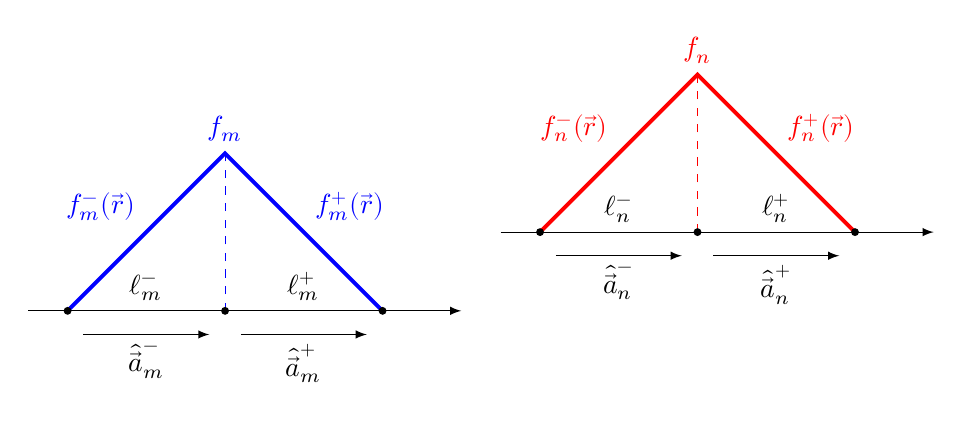
\begin{tikzpicture}[> = latex]
	\draw[->] (-0.5, 0) -- (5, 0);	
	
	\draw[blue, line width=0.5mm] (0, 0) -- node[above left] {$f_m^{-}(\vecr)$} (2, 2) node[above] {$f_m$} -- node[above right] {$f_m^{+}(\vecr)$} (4, 0);
	\draw[blue, dashed] (2, 0) -- (2, 2);
	\node[fill = black, circle, inner sep=0pt, minimum size = 1mm] at (0, 0) {};
	\node[fill = black, circle, inner sep=0pt, minimum size = 1mm] at (2, 0) {};
	\node[fill = black, circle, inner sep=0pt, minimum size = 1mm] at (4, 0) {};
	
	\draw (1, 0) node[above] {$\ell_m^{-}$};
	\draw (3, 0) node[above] {$\ell_m^{+}$};
	
	\draw[->] (0.2, -0.3) -- node[below] {$\hat{\vec{a}}_m^{-}$} (1.8, -0.3);
	\draw[->] (2.2, -0.3) -- node[below] {$\hat{\vec{a}}_m^{+}$} (3.8, -0.3);
	
	
	\draw[->] (5.5, 1) -- (11, 1);	
	
	\draw[red, line width=0.5mm] (6, 1) -- node[above left] {$f_n^{-}(\vecr)$} (8, 3) node[above] {$f_n$} -- node[above right] {$f_n^{+}(\vecr)$} (10, 1);
	\draw[red, dashed] (8, 1) -- (8, 3);
	\node[fill = black, circle, inner sep=0pt, minimum size = 1mm] at (6, 1) {};
	\node[fill = black, circle, inner sep=0pt, minimum size = 1mm] at (8, 1) {};
	\node[fill = black, circle, inner sep=0pt, minimum size = 1mm] at (10, 1) {};
	
	\draw (7, 1) node[above] {$\ell_n^{-}$};
	\draw (9, 1) node[above] {$\ell_n^{+}$};
	
	\draw[->] (6.2, 0.7) -- node[below] {$\hat{\vec{a}}_n^{-}$} (7.8, 0.7);
	\draw[->] (8.2, 0.7) -- node[below] {$\hat{\vec{a}}_n^{+}$} (9.8, 0.7);
\end{tikzpicture}
	\caption{Definition of (non-overlapping) basis functions.}
	\label{fig:mom_basis2}
\end{figure}
\begin{align*}
	A_{mn}^{++} & = \hat{\vec{a}}_m^{+} \cdot \hat{\vec{a}}_n^{+} \frac{\ell_m^{+} \ell_n^{+}}{4} \sum_{p = 1}^M \sum_{q = 1}^M w_p w_q f_m(\vec{r}_p^{+}) f_n(\vec{r}_q^{+}) G(\vec{r}_p^{+}, \vec{r}_q^{+}) \\
	A_{mn}^{+-} & = \hat{\vec{a}}_m^{+} \cdot \hat{\vec{a}}_n^{-} \frac{\ell_m^{+} \ell_n^{-}}{4} \sum_{p = 1}^M \sum_{q = 1}^M w_p w_q f_m(\vec{r}_p^{+}) f_n(\vec{r}_q^{-}) G(\vec{r}_p^{+}, \vec{r}_q^{-}) \\
	A_{mn}^{-+} & = \hat{\vec{a}}_m^{-} \cdot \hat{\vec{a}}_n^{+} \frac{\ell_m^{-} \ell_n^{+}}{4} \sum_{p = 1}^M \sum_{q = 1}^M w_p w_q f_m(\vec{r}_p^{-}) f_n(\vec{r}_q^{+}) G(\vec{r}_p^{-}, \vec{r}_q^{+}) \\
	A_{mn}^{--} & = \hat{\vec{a}}_m^{-} \cdot \hat{\vec{a}}_n^{-} \frac{\ell_m^{-} \ell_n^{-}}{4} \sum_{p = 1}^M \sum_{q = 1}^M w_p w_q f_m(\vec{r}_p^{-}) f_n(\vec{r}_q^{-}) G(\vec{r}_p^{-}, \vec{r}_q^{-})
\end{align*}
Similarly, for the scalar potential contributions. Here, we can pre-calculate the divergence of the basis functions, which is constant over the element (for triangular basis functions).
\begin{align}
	\nabla \cdot \vec{f}_m^{+}(\vecr) & = \frac{-1}{\ell_m^+} \qquad \vecr \in \operatorname{supp}(f_m^+) \\
	\nabla \cdot \vec{f}_m^{-}(\vecr) & = \frac{+1}{\ell_m^-} \qquad \vecr \in \operatorname{supp}(f_m^-)
\end{align}
Therefore, the scalar potential terms become
\begin{align*}
	\Phi_{mn}^{++} & = \frac{-1}{\ell_{m}^{+}} \frac{-1}{\ell_{m}^{+}} \frac{\ell_m^{+} \ell_n^{+}}{4} \sum_{p = 1}^M \sum_{q = 1}^M w_p w_q G(\vec{r}_p^{+}, \vec{r}_q^{+}) \\
	& = \frac{1}{4} \sum_{p = 1}^M \sum_{q = 1}^M w_p w_q G(\vec{r}_p^{+}, \vec{r}_q^{+}) \\
	\Phi_{mn}^{+-} & = -\frac{1}{4} \sum_{p = 1}^M \sum_{q = 1}^M w_p w_q G(\vec{r}_p^{+}, \vec{r}_q^{-}) \\
	\Phi_{mn}^{-+} & = -\frac{1}{4} \sum_{p = 1}^M \sum_{q = 1}^M w_p w_q G(\vec{r}_p^{-}, \vec{r}_q^{+}) \\
	\Phi_{mn}^{--} & = \frac{1}{4} \sum_{p = 1}^M \sum_{q = 1}^M w_p w_q G(\vec{r}_p^{-}, \vec{r}_q^{-})
\end{align*}

\subsubsection{Self Terms}
If the basis functions $n, m$ overlap (see Figure~\ref{fig:mom_basis3}), then we must treat the singularity that arises in the integral of the Green's function. We can do this by evaluating the inner integral analytically, and the outer integral numerically using an $M$-point quadrature rule. Assume that the singularity is in the $++$ direction. For the vector potential term,
\begin{figure}[b]
	\centering
	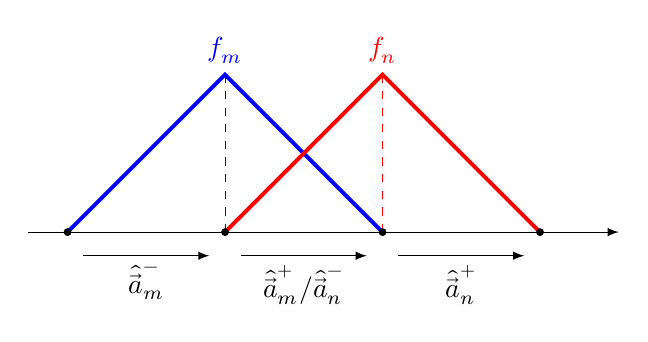
\begin{tikzpicture}[> = latex]
	\draw[->] (-0.5, 0) -- (7, 0);	
	
	\draw[blue, line width=0.5mm] (0, 0) -- (2, 2) node[above] {$f_m$} -- (4, 0);
	\draw[red, line width=0.5mm] (2, 0) -- (4, 2) node[above] {$f_n$} -- (6, 0);
	\draw[blue, dashed] (2, 0) -- (2, 2);
	\draw[red, dashed] (4, 0) -- (4, 2);
	\node[fill = black, circle, inner sep=0pt, minimum size = 1mm] at (0, 0) {};
	\node[fill = black, circle, inner sep=0pt, minimum size = 1mm] at (2, 0) {};
	\node[fill = black, circle, inner sep=0pt, minimum size = 1mm] at (4, 0) {};
	\node[fill = black, circle, inner sep=0pt, minimum size = 1mm] at (6, 0) {};
	
	\draw[->] (0.2, -0.3) -- node[below] {$\hat{\vec{a}}_m^{-}$} (1.8, -0.3);
	\draw[->] (2.2, -0.3) -- node[below] {$\hat{\vec{a}}_m^{+}$/$\hat{\vec{a}}_n^{-}$} (3.8, -0.3);
	\draw[->] (4.2, -0.3) -- node[below] {$\hat{\vec{a}}_n^{+}$} (5.8, -0.3);
\end{tikzpicture}
	\caption{Definition of (overlapping) basis functions.}
	\label{fig:mom_basis3}
\end{figure}
\begin{align*}
	A_{mn}^{++} & = \hat{\vec{a}}_m^{+} \cdot \hat{\vec{a}}_n^{+} \frac{\ell_m^+}{2} \sum_{p = 1}^M w_p f_m(\vec{r}_p^+) \int_{f_n} f_n(\vecrp) G(\vecr_p^+, \vecrp) d\vecrp \\
	& = \hat{\vec{a}}_m^{+} \cdot \hat{\vec{a}}_n^{+} \frac{\ell_m^+}{2} \sum_{p = 1}^M w_p f_m(\vec{r}_p^+) S_1(\vecr_p^+)
\end{align*}
And for the scalar potential term,
\begin{equation*}
	\Phi_{mn}^{++} = \frac{\ell_m^+}{2} \sum_{p = 1}^M w_p \frac{1}{\ell_m^+ \ell_n^+} \int_{f_n} G(\vecr_p^+, \vecrp) d\vecrp  = \frac{\ell_m^+}{2} \sum_{p = 1}^M w_p S_2(\vecr_p^+)
\end{equation*}
where we define $S_1(r)$ and $S_2(r)$ as follows
\begin{align}
	S_1(\vecr) & = \int_{f_n} f_n(\vecrp) G(\vecr, \vecrp) d\vecrp \\
	S_2(\vecr) & = \frac{1}{\ell_m \ell_n} \int_{f_n} G(\vecr, \vecrp) d\vecrp
\end{align}

\subsection{Practical Matrix Assembly per Element}

\subsection{Boundary Conditions}
\label{sec:mom_bc}
Two boundary conditions arise from the equation of charge conservation:
\begin{enumerate}
	\item The basis vectors $\vec{a}_n$ should be oriented such that (\ref{eq:charge_cons}) holds at every node.
	\item A condition $I = 0$ must be imposed on the end-points of every segment, as this is the only way to enforce (\ref{eq:charge_cons}).
\end{enumerate}
\begin{equation}
	\nabla \cdot \vec{J} = 0
	\label{eq:charge_cons}	
\end{equation}

\subsection{Post-processing}

\subsubsection{Antenna impedance}
To calculate the impedance seen by a source embedded in segment $e$, with nodes $n_1, n_2$, we make use of the current coefficient vector $\begin{Bmatrix}
	I
\end{Bmatrix}$. The impedance is defined as
\begin{equation}
	Z = \frac{V_{src}}{I_{src}},
\end{equation}
where $V_{src}$ is the known source voltage and $I_{src}$ is the solved current averaged over segment $e$:
\begin{equation*}
	I_{src} = \frac{1}{2}\left( I[n_1] + I[n_2] \right)
\end{equation*}

\subsubsection{Far-field radiation}
The far-field radiation pattern can also be derived from the solved current vector. The EFIE can be simplified by assuming that the $\nicefrac{1}{r}$ are dominant, and that higher order terms have negligible amplitude in the far field.
\begin{equation}
	\vec{E}(\vecr) = -j\omega\mu \int \vec{J}(\vecrp) G_k(\vecr, \vecrp) d\vecrp
	\label{eq:ff_efie}
\end{equation}
This expression can be further simplified by considering that $\vecr \gg \vecrp$, such that
\begin{equation}
	|\vecr - \vecrp| = \left\{ \begin{array}{ll}
		r \quad & \text{for amplitude variations} \\
		r - \vecrp \cdot \hat{\vecr} \quad & \text{for phase variations}
	\end{array} \right.
	\label{eq:ff_approx}
\end{equation}
where $r = |\vecr|$ and $\hat{\vecr} = \nicefrac{\vecr}{|\vecr|}$. Applying (\ref{eq:ff_approx}) to (\ref{eq:ff_efie}) yields
\begin{equation}
	\vec{E}(\vecr) = j\omega\mu \frac{e^{-j k r}}{4\pi r} \int ((\hat{\vecr} \cdot \vec{J}(\vecrp)) \hat{\vecr} - \vec{J}(\vecrp)) e^{j k \vecrp \cdot \hat{\vecr}} d\vecrp
\end{equation}
Applying the same discretization procedure,
\begin{equation}
	\vec{E}(\vecr) = j\omega\mu \frac{e^{-j k r}}{4\pi r} \sum_{n = 1}^{N} I_n \int_{f_n} ((\hat{\vecr} \cdot \hat{\vec{a}}_n) \hat{\vecr} - \hat{\vec{a}}_n) f_n(\vecrp) e^{j k \vecrp \cdot \hat{\vecr}} d\vecrp
\end{equation}
The integral can be tackled using quadrature and all the terms are known.
	
	\section*{References}
	\begin{itemize}
		\item Gibson, W.C. (2021). The Method of Moments in Electromagnetics (3rd ed.). Chapman and Hall/CRC. \url{https://doi.org/10.1201/9780429355509}
		\item Rothschild, A. (2020). Simulation of a Half-Wave Dipole Designed for 2.5GHz Using the Method of Moments. \url{https://github.com/austinrosh/Wire-Dipole-MoM}
	\end{itemize}
\end{document}
